\documentclass[border=10pt]{standalone}
\usepackage{amsmath}
\usepackage{tikz}
\usetikzlibrary{positioning, arrows.meta, calc, fit, backgrounds, shapes.geometric}
\begin{document}
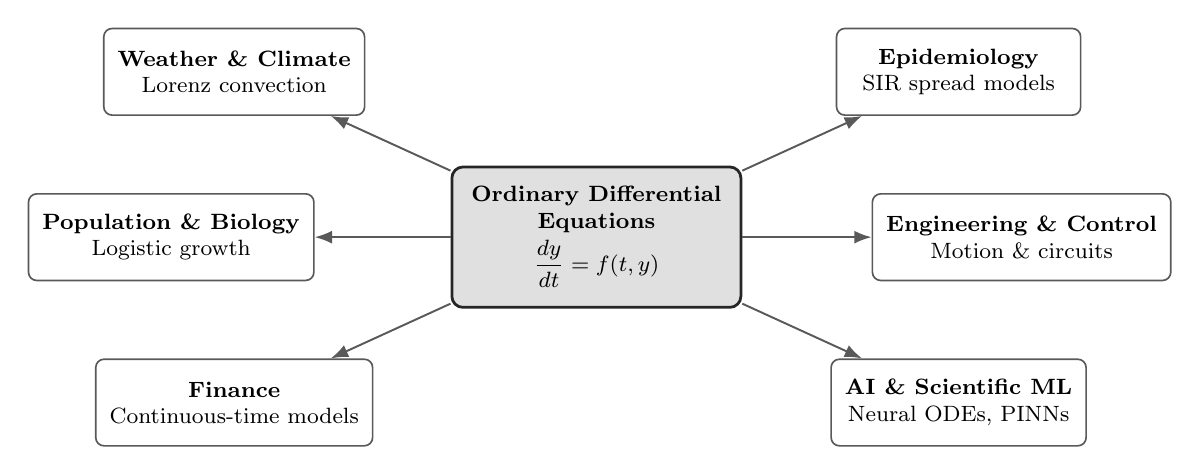
\begin{tikzpicture}[
    font=\footnotesize,
    hub/.style={rounded corners=4pt, draw=black!85, fill=black!12, line width=1.0pt,
                align=center, inner sep=7pt, minimum width=3.4cm, minimum height=1.5cm},
    leaf/.style={rounded corners=3pt, draw=black!65, fill=white, line width=0.6pt,
                 align=center, inner sep=5pt, minimum width=3.1cm, minimum height=1.1cm},
    link/.style={-{Latex[length=2.2mm]}, draw=black!65, line width=0.7pt}
]
\node[hub] (ode) at (0,0) {\textbf{Ordinary Differential}\\\textbf{Equations}\\[2pt]$\dfrac{dy}{dt}=f(t,y)$};
\node[leaf] (weather) at (-4.6, 2.1) {\textbf{Weather \& Climate}\\Lorenz convection};
\node[leaf] (epi)     at ( 4.6, 2.1) {\textbf{Epidemiology}\\SIR spread models};
\node[leaf] (pop)     at (-5.4, 0.0) {\textbf{Population \& Biology}\\Logistic growth};
\node[leaf] (ctrl)    at ( 5.4, 0.0) {\textbf{Engineering \& Control}\\Motion \& circuits};
\node[leaf] (fin)     at (-4.6,-2.1) {\textbf{Finance}\\Continuous-time models};
\node[leaf] (ai)      at ( 4.6,-2.1) {\textbf{AI \& Scientific ML}\\Neural ODEs, PINNs};
\foreach \n in {weather,epi,pop,ctrl,fin,ai}{\draw[link] (ode)--(\n);}
\end{tikzpicture}
\end{document}
